\documentclass[compress]{beamer}        % [compress] (written before {beamer} <=> navigation bar one line, all subsections in 1 line instead of 2

% Setup appearance:
\usetheme{CambridgeUS}
%	AnnArbor | Antibes | Bergen |
%	Berkeley | Berlin | Boadilla |
%	boxes | CambridgeUS | Copenhagen |
%	Darmstadt | default | Dresden |
%	Frankfurt | Goettingen |Hannover |
%	Ilmenau | JuanLesPins | Luebeck |
%	Madrid | Malmoe | Marburg |
%	Montpellier | PaloAlto | Pittsburgh |
%	Rochester | Singapore | Szeged |
%	Warsaw
%

\useoutertheme[footline=authorinstitute,subsection=false]{miniframes}
\usecolortheme{whale}

%	albatross | beaver | beetle |
%	crane | default | dolphin |
%	dove | fly | lily | orchid |
%	rose |seagull | seahorse |
%	sidebartab | structure |
%	whale | wolverine


\setbeamertemplate{footline}
{
  \hbox{%
  \begin{beamercolorbox}[wd=.25\paperwidth,ht=2.25ex,dp=1ex,center]{title in head/foot}%
    \usebeamerfont{date in head/foot}\insertshortauthor
  \end{beamercolorbox}%
  \begin{beamercolorbox}[wd=.5\paperwidth,ht=2.25ex,dp=1ex,center]{date in head/foot}%
    \usebeamerfont{title in head/foot}\insertshortinstitute
  \end{beamercolorbox}%
  \begin{beamercolorbox}[wd=.25\paperwidth,ht=2.25ex,dp=1ex,center]{title in head/foot}%
    \usebeamerfont{date in head/foot}
    \insertframenumber{} / \inserttotalframenumber
    %\insertframenumber{} / \insertpresentationendpage
  \end{beamercolorbox}}%
  \vskip0pt%
}

%\setbeamercolor{titlelike}{parent=structure}
%\setbeamercolor{structure}{fg=beamer@blendedblue}
%% \useinnertheme{rounded}
%\setbeamerfont{block title}{size={}}
%\usefonttheme[onlylarge]{structurebold}   % title and words in the table of contents bold
%\setbeamerfont*{frametitle}{size=\normalsize,series=\bfseries}
\setbeamertemplate{navigation symbols}{}
\setbeamercolor{frametitle}{parent=boxes, bg=white}
{ % only on titlepage


\usepackage{times}
\usepackage{amsmath,amssymb,amsthm}
\usepackage{color}
\usepackage{changepage}
\usepackage{multirow}
\usepackage[absolute,overlay]{textpos}
\usepackage{enumerate}
%\usepackage{pgfpages}
\usepackage[all]{xy}
\usepackage{textcomp}
\usepackage{etex}
\usepackage{tikz}
\usetikzlibrary{shapes}
%\usepackage{handoutWithNotes}
%\pgfpagesuselayout{4 on 1}[border shrink=1mm]




\definecolor{camblue}{RGB}{26,26,89}
\definecolor{Rblue}{RGB}{0,255,255}
\definecolor{Rdarkblue}{RGB}{0,0,255}
\definecolor{Rgreen}{RGB}{0,205,0}
\definecolor{green2}{RGB}{51,204,51}
\newcommand{\tcb}{\textcolor{beamer@blendedblue}}
\newcommand{\tcbb}{\textcolor{camblue}}
\newcommand{\tcr}{\textcolor{red}}
\newcommand{\tcg}{\textcolor{gray}}
\newcommand{\tcgr}{\textcolor{green2}}
\newcommand{\tcblk}{\textcolor{black}}
\newcommand{\tcRg}{\textcolor{Rgreen}}
\newcommand{\tcRdb}{\textcolor{Rdarkblue}}
\newcommand{\tcRb}{\textcolor{Rblue}}
\newcommand{\tcw}{\textcolor{white}}
\newcommand{\m}{\phantom{-}}
\newcommand{\bp}{\tcbb{$\bullet$}\:}


\title{{\huge Statistics for Computing\\[0.1cm]MA4413}}
\author[Kevin Burke]{{\bf\\[0.5cm]{\huge Lecture 9}\\[0.2cm]\emph{The Exponential Distribution and Queueing Theory}\\[1.4cm]Kevin Burke}\\[0.3cm]\tcb{kevin.burke@ul.ie}}

\institute[University of Limerick, Maths \& Stats Dept]{}
\date{}

%\TPGrid[5mm,5mm]{1}{1}

\begin{document}


\begin{frame}[t]
\titlepage
\end{frame}



\section{Exponential Distribution}
\subsection{No Poisson Events in $t$ Intervals}
\begin{frame}{\bf \tcb{No Poisson Events in $t$ Intervals}}
We saw in Lecture8 that
\begin{align*}
X &\sim \text{Poisson}(\lambda) \text{ in 1 interval}.\\[0.3cm]
\Rightarrow X &\sim \text{Poisson}(\lambda\,t) \text{ in $t$ intervals}.\\
\end{align*}

The probability that there are \emph{no events} in $t$ intervals (of time) is:\\[-0.5cm]
\begin{align*}
\Pr(X = 0) = \frac{(\lambda\,t)^0}{0\,!}\,e^{-\lambda\,t} = \frac{1}{1} \,e^{-\lambda\,t} = e^{-\lambda\,t}.\\[-0.2cm]
\end{align*}
No event in $t$ intervals of time $\Rightarrow$ it happens sometime after this.\\[0.3cm]
Thus, $\Pr(X=0)$ is the probability that the event \emph{time} is greater than $t$.
\end{frame}

\subsection{Exponential Distribution}
\begin{frame}{\bf \tcb{Exponential Distribution}}
$X$ is the number of events in an interval of time.\\[0.6cm]

Now let $T$ be the random variable representing the \emph{waiting time} between Poisson events. Note that $T$ $\sim$ {\bf exponential distribution}.\\[0.6cm]

From the previous slide we have that
\begin{align*}
\Pr(T > t) = \Pr(X = 0) = e^{-\lambda\,t}.
\end{align*}
This is the probability function for the exponential distribution.\\[0.7cm]
{\footnotesize(recall that the Poisson distribution also applies to intervals other than time, e.g., distance / area etc. In such cases $T$ is the distance / space between Poisson events)}

\end{frame}



\subsection{Exponential Distribution}
\begin{frame}{\bf \tcb{Exponential Distribution}}
The {\bf exponential distribution} is used for calculating the probability of waiting more than $t$ units of time / distance / space for a Poisson event:
\begin{align*}
\boxed{T \sim \text{Exponential}(\lambda)}
\end{align*}
\begin{align*}
\boxed{\Pr(T > t) = e^{-\lambda\,t}}\\[-1cm]
\end{align*}
\begin{align*}
\text{where } \boxed{t \in [0,\infty)} \text{ is \emph{continuous}}
\end{align*}
\begin{align*}
\boxed{E(T) = \frac{1}{\lambda}}
\end{align*}
\begin{align*}
\boxed{Var(T) = \frac{1}{\lambda^2}}\\[-0.5cm]
\end{align*}

\end{frame}

\section{Continuous Vs Discrete}
\subsection{Continuous Vs Discrete Distributions}
\begin{frame}{\bf \tcb{Continuous  Vs Discrete Distributions}}
The exponential distribution is {\bf continuous} (i.e., the random variable $T$ is continuous) unlike the Binomial and Poisson distributions which are \emph{discrete}.\\[0.6cm]

We \emph{never} calculate ``equal to'' probabilities for continuous distributions!\\[0.1cm]{\footnotesize(recall from Lecture8 that the probability of a system crashing at any precise moment in time is zero, i.e., $\Pr(T = t) = 0$)}\\[0.6cm]

Instead, we calculate the probability that $T$ is greater than or less than some value or the probability that $T$ lies in some range of values.\\[0.6cm]

$\Rightarrow$ The probability function used in the exponential case is $\Pr(T > t)$.

\end{frame}



\subsection{Continuous Vs Discrete Distributions}
\begin{frame}{\bf \tcb{Continuous  Vs Discrete Distributions}}

For discrete variables we had $\Pr(X > 1) = \Pr(X \ge 2)$, i.e., the next \emph{discrete} number after 1 is 2.\\[0.8cm]

For \emph{continuous} variables there is really no ``next number''. Think about values such as $1 + 0.01$, $1 + 0.00001$, $1 + 10^{-10}$, $1 + 10^{-1000}$\ldots\\[0.2cm]

Clearly the next continuous number after 1 is indistinguishable from 1\\[0.2cm]
$\Rightarrow$ $\Pr(T > 1) = \Pr(T \ge 1)$.\\[0.9cm]

We make \emph{no distinction} between ``$>$'' and ``$\ge$'' in the continuous case.%\\[0.4cm]

%But don't forget that there \emph{is} a difference in the discrete cases! (Binomial and Poisson)
\end{frame}


\subsection{Discrete}
\begin{frame}{\bf \tcb{Discrete}\\[-1.1cm]}
\begin{center}
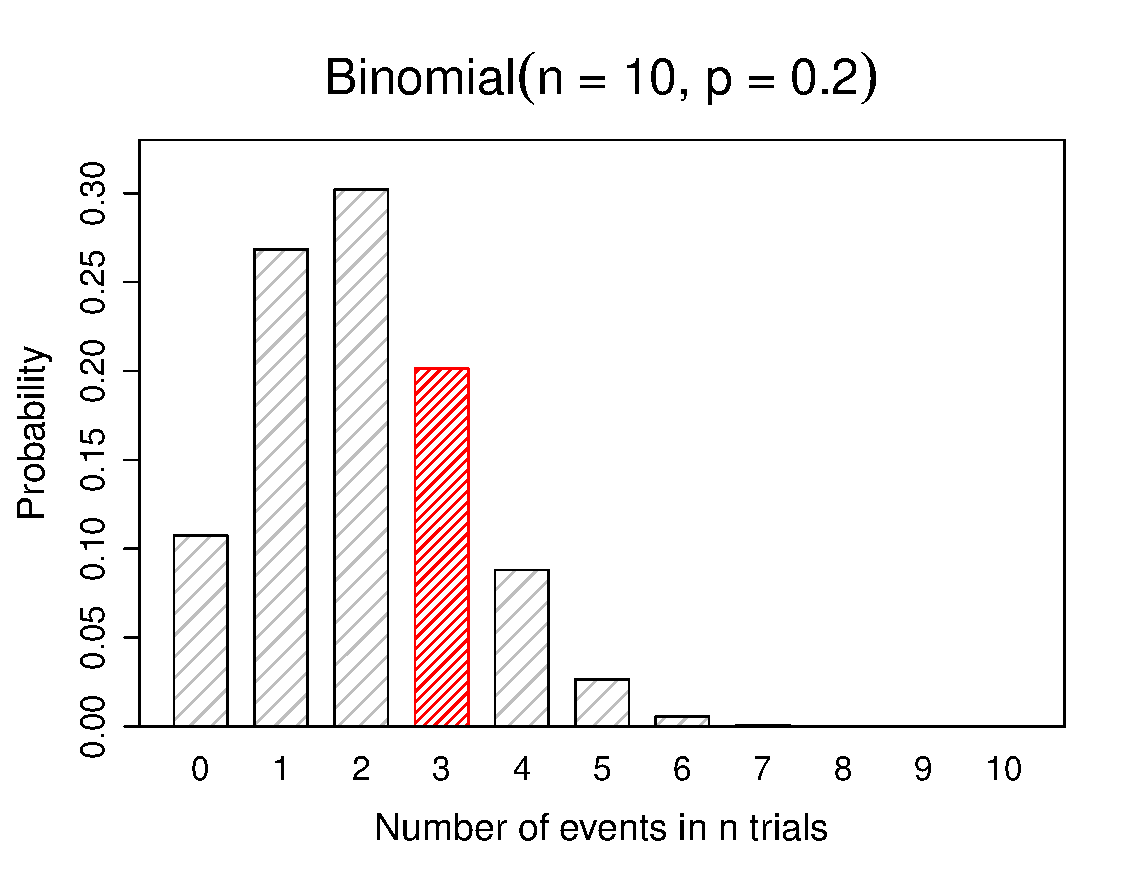
\includegraphics[width=0.87\textwidth, trim = 0.0cm 0.5cm 0.3cm 0.5cm, clip]{Binomial}
\end{center}
\begin{textblock}{1}(6.3,7.6)
\xymatrixcolsep{0.8cm}
\xymatrix{&\ar@/^0.4pc/@{-}[ld]\\&}
\end{textblock}
\begin{textblock}{10}(5,6.8)
\begin{scriptsize}
\begin{align*}
\Pr(X=3) &= \binom{10}{3} \, 0.2^3 \, 0.8^{7}\\
&= 0.2013.
\end{align*}
\end{scriptsize}
\end{textblock}
\end{frame}


\subsection{Discrete}
\begin{frame}{\bf \tcb{Discrete}\\[-1.1cm]}
\begin{center}
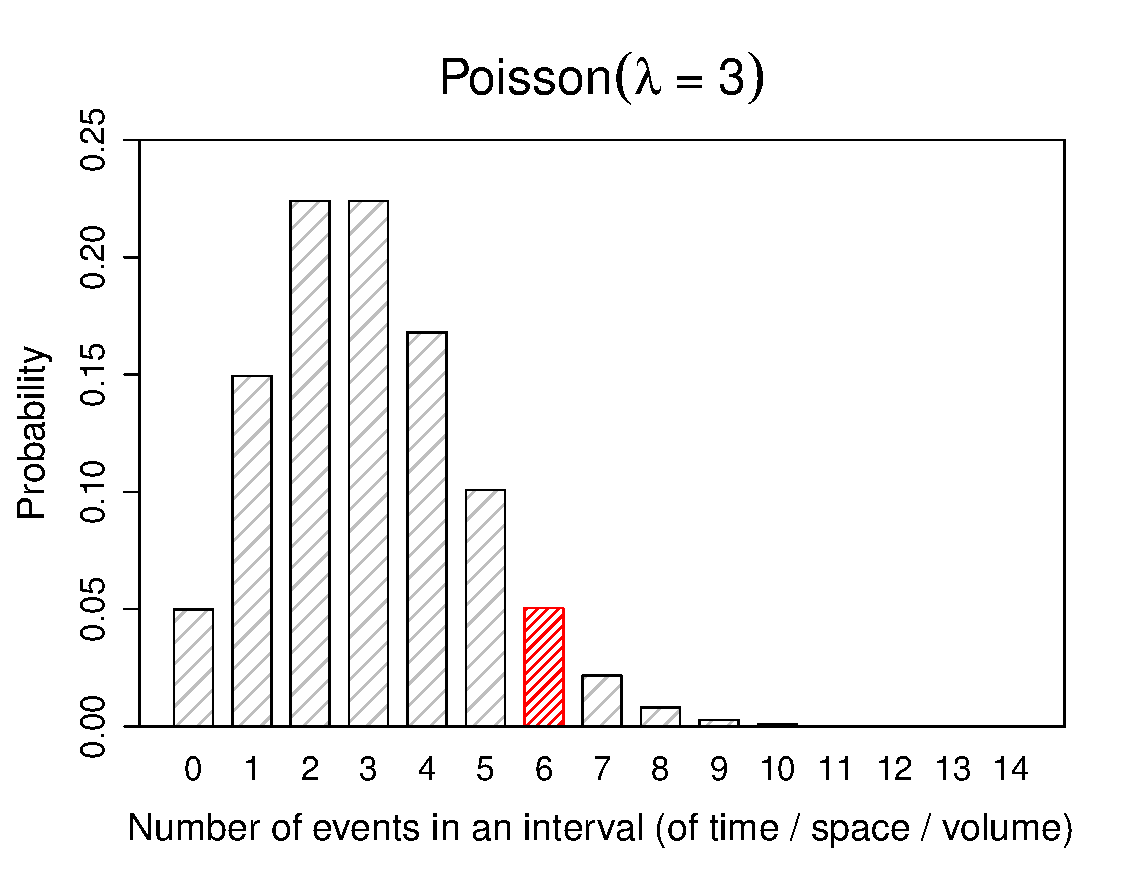
\includegraphics[width=0.87\textwidth, trim = 0.0cm 0.5cm 0.3cm 0.5cm, clip]{Poisson}
\end{center}
\begin{textblock}{1}(7.45,9.8)
\xymatrixcolsep{1cm}
\xymatrix{&\ar@/^0.4pc/@{-}[ld]\\&}
\end{textblock}
\begin{textblock}{10}(5.6,8.5)
\begin{scriptsize}
\begin{align*}
\Pr(X=6) &= \frac{3^6}{6\,!}\,e^{-3}\\
&= 0.0504.
\end{align*}
\end{scriptsize}
\end{textblock}
\end{frame}



\subsection{Continuous}
\begin{frame}{\bf \tcb{Continuous}\\[-1.1cm]}\label{expplot}
\begin{center}
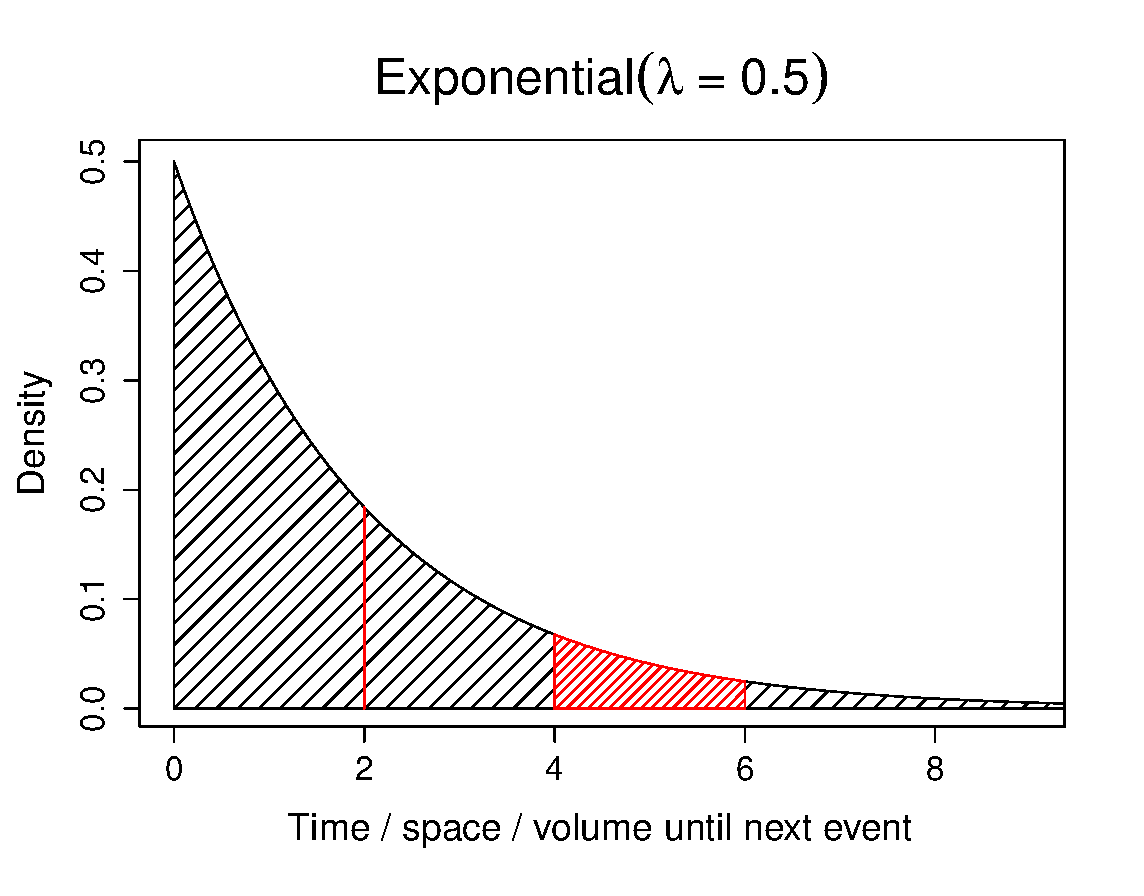
\includegraphics[width=0.87\textwidth, trim = 0.0cm 0.5cm 0.3cm 0.5cm, clip]{Exponential}
\end{center}
\begin{textblock}{1}(8,10.5)
\xymatrixcolsep{0.7cm}
\xymatrix{&\ar@/^0.6pc/@{-}[ld]\\&}
\end{textblock}
\begin{textblock}{10}(5.6,9.4)
\begin{scriptsize}
\begin{align*}
\Pr(4<T<6) &= \Pr(T > 4) - \Pr(T > 6) \\
&= e^{-0.5(4)} - e^{-0.5(6)} \\&= 0.0855.
\end{align*}
\end{scriptsize}
\end{textblock}
\begin{textblock}{1}(5.35,8)
\xymatrixcolsep{1cm}
\xymatrix{&\ar@/^1pc/@{-}[ldd]\\&\\&}
\end{textblock}
\begin{textblock}{10}(2.6,7.2)
\begin{scriptsize}
\begin{align*}
\Pr(T=2) &= 0.
\end{align*}
\end{scriptsize}
\end{textblock}
\end{frame}

\subsection{Continuous}
\begin{frame}{\bf \tcb{Continuous}\\[-1.1cm]}\label{normplot}
\begin{center}
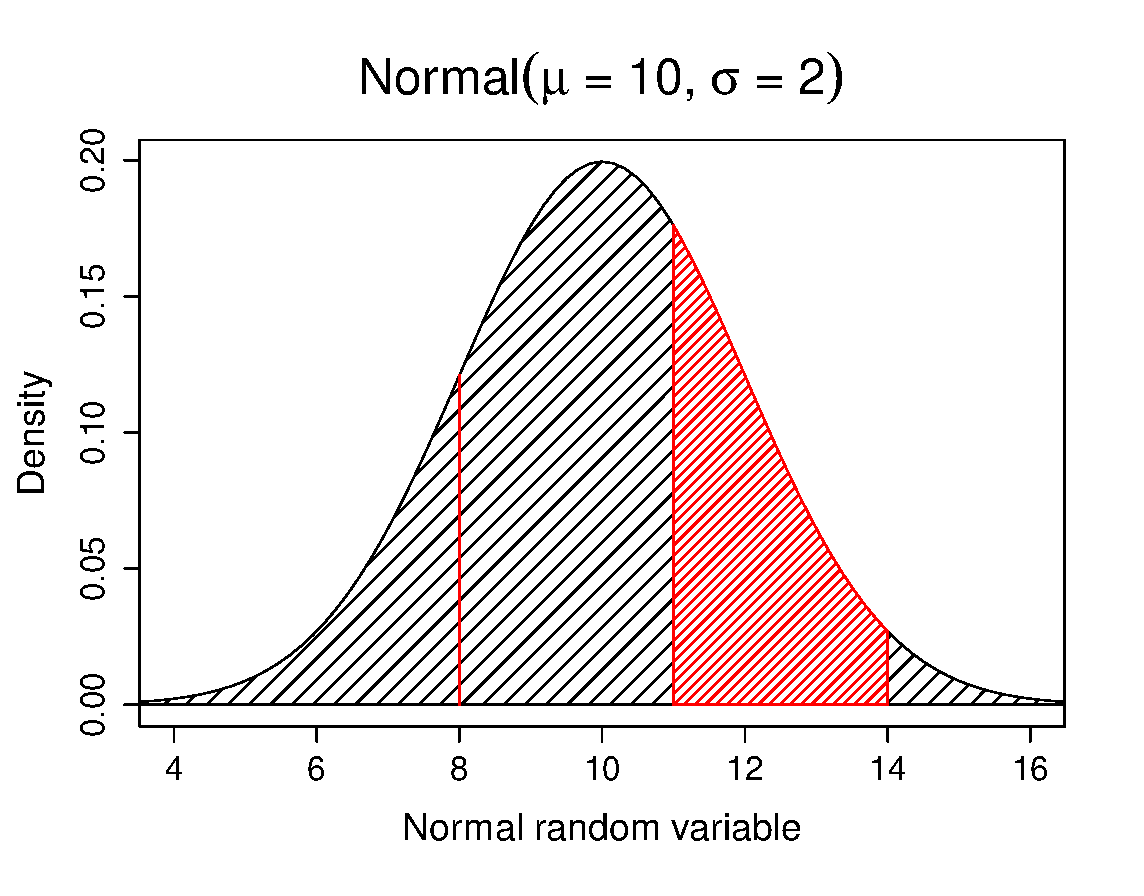
\includegraphics[width=0.87\textwidth, trim = 0.0cm 0.5cm 0.3cm 0.5cm, clip]{Normal}
\end{center}
\begin{textblock}{1}(10.1,8)
\xymatrixcolsep{0.8cm}
\xymatrix{&\ar@/^0.7pc/@{-}[ld]\\&}
\end{textblock}
\begin{textblock}{10}(7.3,7)
\begin{scriptsize}
\begin{align*}
&\Pr(11<X<14) \\ %&= \Pr(X>11) - \Pr(X>14)\\
&\qquad\quad= 0.2858.\\
&\qquad\text{{\tiny(normal tables used)}}
\end{align*}
\end{scriptsize}
\end{textblock}
\begin{textblock}{1}(5.25,8)
\xymatrixcolsep{1cm}
\xymatrix{\ar@/_1pc/@{-}[rdd]&\\&\\&}
\end{textblock}
\begin{textblock}{10}(-0.2,7.2)
\begin{scriptsize}
\begin{align*}
\Pr(X=8) &= 0.
\end{align*}
\end{scriptsize}
\end{textblock}
\end{frame}




\section{Exponential Examples}
\subsection{Example: System Crash Time}
\begin{frame}{\bf \tcb{Example: System Crash Time}}
The number of system crashes in a year is  $X \sim \text{Poisson}(\lambda=3)$.\\[0.2cm]
$\Rightarrow$ the \emph{time between} system crashes is $T \sim \text{Exponential}(\lambda=3)$.\\[0.2cm]
$\Rightarrow$ $\Pr(T > t) = e^{-3\,t}$.\\[0.9cm]

What is the probability that the system works for more than 6 months (i.e., 0.5 years) without a crash?\\[0.5cm]
In other words, we wait more than 0.5 years for the next crash:\\[-0.3cm]
\begin{align*}
\Pr(T>0.5) = e^{-3(0.5)} = e^{-1.5} = 0.2231.
\end{align*}

\end{frame}


\subsection{Example: System Crash Time}
\begin{frame}{\bf \tcb{Example: System Crash Time}}
What is the probability that the next crash happens within 3 months?\\[0.3cm]
In other words, we wait less than $\frac{3}{12} = 0.25$ years for the next crash:\\
\begin{align*}
\Pr(T<0.25) &= 1-\Pr(T\ge0.25) \tag{$\ge$ the same as $>$}\\[0.2cm]
&= 1-\Pr(T>0.25) \tag{since $T$ is continuous}\\[0.2cm]
&= 1-e^{-3(0.25)} \\[0.2cm]
&= 1-0.4724  \\[0.2cm]
&= 0.5276.
\end{align*}

\end{frame}


\subsection{Example: System Crash Time}
\begin{frame}{\bf \tcb{Example: System Crash Time}}\label{expexampletab}
What is the probability that the next crash occurs between 6 months and 1 year from now.\\[-0.4cm]
\begin{align*}
\Pr(0.5<T<1) &= \Pr(T>0.5) - \Pr(T>1) \\[0.2cm]
&= e^{-3(0.5)} - e^{-3(1)}\\[0.2cm]
&= e^{-1.5} - e^{-3}\\[0.2cm]
&= 0.2231 - 0.0498 \\[0.2cm]
&= 0.1733.
\end{align*}

\end{frame}




\subsection{Example: System Crash Time}
\begin{frame}{\bf \tcb{Example: System Crash Time}}
What is the \emph{average} waiting time?\\[-0.4cm]
\begin{align*}
E(T) = \frac{1}{\lambda} = \frac{1}{3} \text{ years},
\end{align*}
i.e.,  on average we wait $(\frac{1}{3}\times12 =)\,\, 4$ months for a crash. This should make sense as there are 3 crashes per year.\\[0.5cm]

What is the standard deviation of $T$?\\[-0.6cm]
\begin{align*}
Var(T) &= \frac{1}{\lambda^2} = \frac{1}{9} \text{ years$^2$}.\\[0.4cm]
Sd(T) &= \sqrt{\frac{1}{9}} = \frac{1}{3} \text{ years}.
\end{align*}


\end{frame}




\subsection{Example: Laptop Battery Life}
\begin{frame}{\bf \tcb{Example: Laptop Battery Life}}
Note: \emph{Often you have $E(T)$ and need to calculate $\lambda$.}\\[0.5cm]


Let's assume that the battery life of a laptop has an exponential distribution with a mean of 3 hours, i.e., $E(T) = 3$.\\[0.5cm]

We know that $E(T) = \frac{1}{\lambda}$ from which we find that:
\begin{align*}
\boxed{\lambda = \frac{1}{E(T)}}.\\
\end{align*}

Laptop battery life is $T \sim \text{Exponential}(\lambda = \frac{1}{3})$ and, the probability function is $\Pr(T > t) = e^{-\frac{1}{3}\,t}$.
\end{frame}






\subsection{Question 1}
\begin{frame}{\bf \tcb{Question 1}}
The \emph{average time} between customers arriving to a shop is 5 minutes. We will assume that the time, $T$, has an exponential distribution. Calculate the following:\\[0.2cm]
\begin{enumerate}[a)]\itemsep0.3cm
\item The average arrival \emph{rate}, i.e., $\lambda$ customers per minute.
\item The probability that we wait more than 15 minutes for the next customer.
\item The probability that the next customer arrives within 1 minute.
\item The average \emph{number of customers} in a 1 hour period. What is the standard deviation that goes with this average?
\item The probability that \emph{15 or more} customers arrive in a 1 hour period.
\end{enumerate}

\end{frame}




\subsection{R Code}
\begin{frame}{\bf \tcb{R Code}}
For the exponential distribution we calculate \emph{greater than} probabilities, i.e., $\Pr(T > t)$. Note that \texttt{rate} $= \lambda$.\\[0.4cm]

\begin{tabular}{|l|}
\hline
Examples: \\[0.2cm]
\texttt{pexp(0.5,rate=3,lower=F)} \\
gives \texttt{0.2231302}.\\[0.2cm]
\texttt{pexp(1,rate=3,lower=F)} \\
gives \texttt{0.04978707}.\\[0.2cm]
\hline
\multicolumn{1}{c}{}\\[0.0cm]
\end{tabular}

Compare this with slide \pageref{expexampletab}.\\[0.6cm]

{\footnotesize(Warning: although there is also a \texttt{dexp} function, it differs from \texttt{dbinom} or \texttt{dpois} since it does not give $\Pr(T=t)$. The values produced by \texttt{dexp} are called \emph{density} points - this fact is alluded to on slides \pageref{expplot} and \pageref{normplot})}
\end{frame}




\subsection{R Code}
\begin{frame}{\bf \tcb{R Code}}
We can \emph{generate} exponential random variables as follows:\\[0.5cm]

\begin{tabular}{|l|}
\hline
Example: \\[0.2cm]
\texttt{rexp(100,rate=3)} \\
generates 100 Exponential$(\lambda=3)$ variables.\\
\hline
\multicolumn{1}{c}{}\\[0.2cm]
\end{tabular}


\end{frame}





\section{Queueing Theory\hspace{0.2cm}}
\subsection{Queueing Theory}
\begin{frame}{\bf \tcb{Queueing Theory}}
The theory of \emph{Poisson arrivals} and \emph{exponential waiting times} is useful in the study of {\bf queues} (i.e., waiting lines).\\[0.4cm]

Examples:\\
\begin{itemize}\itemsep0.2cm
\item {\bf Customers waiting to be served}.
\item Jobs waiting to be processed.
\item Planes waiting to land.
\item Objects manufactured on a factory line.
\item Traffic at a busy junction.\\
\end{itemize}

\end{frame}


\subsection{Definitions and Notation}
\begin{frame}{\bf \tcb{Definitions and Notation}}

\begin{itemize}\itemsep0.5cm
\item The {\bf system} is the \emph{whole} system, i.e., \emph{queue + service}.
\item  $\lambda_a$ is the {\bf arrival rate} to the system.
\item  $\lambda_s$ is the {\bf service rate} \emph{within} the system.
\item  $N$ is the {\bf total number} of customers in the system.
\item  $T$ is the  {\bf total time} that a customer spends in the system.\\[0.8cm]
\end{itemize}


Important note: we require that $\boxed{\lambda_a < \lambda_s}$  to prevent the system from becoming overloaded with customers.
\end{frame}



\subsection{Little's Law (1961)}
\begin{frame}{\bf \tcb{Little's Law (1961)}}

{\bf Little's Law} is fundamental to the theory of queueing since it holds for \emph{almost any queueing system} (or component of a system):\\
\begin{align*}
\boxed{E(N) = \lambda_a \, E(T)},\\[-0.3cm]
\end{align*}
i.e., the expected number of customers in a system is the rate at which they arrive multiplied by the expected time spent in the system.\\[1cm]

Example: people arrive to a museum at a rate of $\lambda_a = 30$ per hour and spend $E(T) = 1.5$ hours there on average $\Rightarrow$ the average number of people in the museum is $E(N) = \lambda_a \, E(T) = 30(1.5) = 45$.
\end{frame}



\subsection{Utilisation Factor}
\begin{frame}{\bf \tcb{Utilisation Factor}}
The {\bf utilisation factor} or \emph{traffic intensity} measures the load on the service component:\\[-0.4cm]
\begin{align*}
\boxed{\rho = \frac{\lambda_a}{\lambda_s}}.\\[-0.6cm]
\end{align*}
{\footnotesize(note: $\rho$ is the Greek letter ``rho'')}\\[0.3cm]

It is the proportion of time that the server is busy. It should be clear that $\lambda_a$ must be smaller than $\lambda_s$ or the system becomes overloaded.\\[0.6cm]

Example: customers arrive at a rate of 1 per minute; the server can deal with 4 customers per minute. Thus, $\rho = 1/4 = 0.25:$ the server is \emph{busy} 25\% of the time and \emph{idle} 75\% of the time.

\end{frame}




\subsection{$M / M / 1$ System}
\begin{frame}{\bf \tcb{$M / M / 1$ System\\[-1.5cm]}}

\begin{align*}
\xymatrixcolsep{0.5cm}
\xymatrix{\lambda_a \ar@{->}[r] & \hspace{-0.1cm}
{\begin{tabular}{@{}c|@{}c|@{}c|@{}c|@{}c|@{}c}
\cline{1-5}
&&&& &
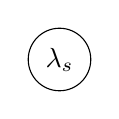
\begin{tikzpicture}[baseline=(char.base)]
\node(char)[draw,shape=circle]{$\lambda_s$};
\end{tikzpicture}\\
\cline{1-5}
\end{tabular}} \hspace{-0.3cm}\ar@{->}[r] & %\lambda_a
}
\end{align*}
The {\boldmath$M / M / 1$} is the simplest queue structure. It is a \emph{first in first out} queue which consists of:\\[0.1cm]
\begin{enumerate}\itemsep0.5cm
\item[{\boldmath$M$}] The arrival process is \emph{memoryless}: customer arrivals are \emph{independent} according to a Poisson$(\lambda_a)$ distribution.
\item[{\boldmath$M$}] The service process is \emph{memoryless}: service times are \emph{independent} according to an Exponential$(\lambda_s)$ distribution.
\item[{\boldmath$1$}] There is one service node, i.e., only one customer can be served at any given time.\\[0.6cm]
\end{enumerate}

Of course we must have $\lambda_a < \lambda_s$.

\end{frame}





\subsection{$M / M / 1$ System}
\begin{frame}{\bf \tcb{$M / M / 1$ System}}

\begin{textblock}{1}(6.5,2.5)
\xymatrixrowsep{0.5cm}
\xymatrixcolsep{0.6cm}
\xymatrix{\ar@/_0.3pc/@{.}[rd]&\\&}
\end{textblock}
\begin{textblock}{8}(5.2,2.3)
\begin{scriptsize}
Queue Component \,\, + \,\, Service Node \,\, = \,\, System
\end{scriptsize}
\end{textblock}
\begin{textblock}{1}(8.8,2.5)
\xymatrixrowsep{0.5cm}
\xymatrixcolsep{0.6cm}
\xymatrix{&\ar@/^0.3pc/@{.}[ld]\\&}
\end{textblock}
\begin{textblock}{1}(8.8,4.7)
\xymatrixrowsep{0.5cm}
\xymatrixcolsep{0.6cm}
\xymatrix{&\\ & \ar@/^0.5pc/@{.}[lu]}
\end{textblock}
\begin{textblock}{3}(9.3,6)
\begin{scriptsize}
Service rate
\end{scriptsize}
\end{textblock}
\begin{textblock}{1}(5,4.6)
\xymatrixrowsep{0.5cm}
\xymatrixcolsep{0.4cm}
\xymatrix{&\\ \ar@/_0.5pc/@{.}[ru]& }
\end{textblock}
\begin{textblock}{3}(3.4,5.6)
\begin{scriptsize}
Arrival rate
\end{scriptsize}
\end{textblock}


\begin{align*}
\xymatrixcolsep{0.5cm}
\xymatrix{\lambda_a \ar@{->}[r] & \hspace{-0.1cm}
{\begin{tabular}{@{}c|@{}c|@{}c|@{}c|@{}c|@{}c}
\cline{1-5}
&&&& &
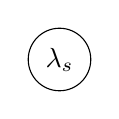
\begin{tikzpicture}[baseline=(char.base)]
\node(char)[draw,shape=circle]{$\lambda_s$};
\end{tikzpicture}\\
\cline{1-5}
\end{tabular}} \hspace{-0.3cm}\ar@{->}[r] & %\lambda_a
}\\[0.3cm]
\end{align*}


\begin{itemize}\itemsep0.5cm
\item {\bf Number of arrivals: {\boldmath$X_a \sim \text{Poisson}(\lambda_a)$}} \quad {\footnotesize$\Leftrightarrow$ $T_a \sim \text{Exponential}(\lambda_a)$}\newline
    \phantom{{\bf Number of arrivals: {\boldmath$X_a \sim \text{Poisson}(\lambda_a)$}}} \qquad {\footnotesize(time between arrivals)}
\item {\bf Service times: {\boldmath$T_s \sim \text{Exponential}(\lambda_s)$}} \quad {\footnotesize$\Leftrightarrow$ $X_s \sim \text{Poisson}(\lambda_s)$}\newline
    \phantom{{\bf Service times: {\boldmath$T_s \sim \text{Exponential}(\lambda_s)$}}} \qquad {\footnotesize(service ``potential''}
    \phantom{{\bf Service times: {\boldmath$T_s \sim \text{Exponential}(\lambda_s)$}}} \qquad\qquad{\footnotesize - \emph{not important!})}
\item Note that {\boldmath$\lambda_a < \lambda_s$}
\end{itemize}


\end{frame}



\subsection{$M / M / 1$ Results}
\begin{frame}{\bf \tcb{$M / M / 1$ Results}}
Based on theory of \emph{birth-death processes} (i.e., arrival-departure) one can derive that the time a customer spends in the system is:
\begin{align*}
\boxed{T \sim \text{Exponential}(\lambda_s - \lambda_a)}.
\end{align*}
Thus, we know that $\Pr(T > t) = e^{-(\lambda_s - \lambda_a)\,t}$ and also
\begin{align*}
\boxed{E(T) = \frac{1}{\lambda_s - \lambda_a}}.
\end{align*}

Little's Law gives us the expected number of customers in the system:
\begin{align*}
\boxed{E(N) = \lambda_a \, E(T) = \frac{\lambda_a}{\lambda_s - \lambda_a}}.
\end{align*}

\end{frame}




\subsection{$M / M / 1$ Results}
\begin{frame}{\bf \tcb{$M / M / 1$ Results}}

We had that service time is $T_s \sim \text{Exponential}(\lambda_s) \Rightarrow E(T_s) = \frac{1}{\lambda_s}$.\\[0.5cm]


Now let $T_q$ represent the time spent in the \emph{queue component only}.\\[0.5cm]


It should be clear that $E(T) = E(T_q) + E(T_s)$. Thus, the expected time waiting in the queue is
\begin{align*}
\boxed{E(T_q) = E(T) - E(T_s)},
\end{align*}
and from Little's Law the expected number of customers in the queue is $E(N_q) = \lambda_a \, E(T_q)$.\\[0.5cm]

{\footnotesize(note: it turns out that, unlike $T$ and $T_s$, the time waiting in the queue component, $T_q$, does \emph{not} have an exponential distribution)}

\end{frame}




\subsection{Burke's Theorem (1956)}
\begin{frame}{\bf \tcb{Burke's Theorem (1956)}}
Burke's Theorem states that for any $M / M / k$ system, the {\bf number of departures} has the same {\bf Poisson{\boldmath$(\lambda_a)$}} distribution as the arrivals:
\begin{align*}
\xymatrixcolsep{0.5cm}
\xymatrix{\lambda_a \ar@{->}[r] & \hspace{-0.1cm}
{\begin{tabular}{@{}c|@{}c|@{}c|@{}c|@{}c|@{}c}
\cline{1-5}
&&&& &
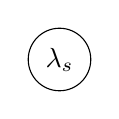
\begin{tikzpicture}[baseline=(char.base)]
\node(char)[draw,shape=circle]{$\lambda_s$};
\end{tikzpicture}\\
\cline{1-5}
\end{tabular}} \hspace{-0.3cm}\ar@{->}[r] & \tcr{\lambda_a}
}
\end{align*}
Note: departures are customers served or \emph{jobs completed}.\\[0.4cm]

The above result is intuitive since:\\[0.1cm]
\begin{itemize}\itemsep0.3cm
\item If \emph{less} customers depart the system than enter: the system is overloaded and the queue is growing infinitely.
\item If \emph{more} customers depart the system than enter: where did these extra customers come from??
\end{itemize}


\end{frame}



\subsection{Tandem Queues}
\begin{frame}{\bf \tcb{Tandem Queues}}

A tandem queue is a finite chain of queues where each customer must visit each one in order:

\begin{align*}
\xymatrixcolsep{0.5cm}
\xymatrix{\lambda_a \ar@{->}[r] & \hspace{-0.1cm}
{\begin{tabular}{@{}c|@{}c|@{}c|@{}c|@{}c|@{}c}
\cline{1-5}
&&&& &
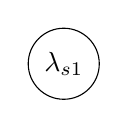
\begin{tikzpicture}[baseline=(char.base)]
\node(char)[draw,shape=circle]{$\lambda_{s1}$};
\end{tikzpicture}\\
\cline{1-5}
\end{tabular}} \hspace{-0.3cm}\ar@{->}[r] & \lambda_a \ar@{->}[r] & \hspace{-0.1cm}
{\begin{tabular}{@{}c|@{}c|@{}c|@{}c|@{}c|@{}c}
\cline{1-5}
&&&& &
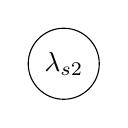
\begin{tikzpicture}[baseline=(char.base)]
\node(char)[draw,shape=circle]{$\lambda_{s2}$};
\end{tikzpicture}\\
\cline{1-5}
\end{tabular}} \hspace{-0.3cm}\ar@{->}[r] & \lambda_a \ar@{->}[r] & \hspace{0.1cm} \ldots
}
\end{align*}

Burke's theorem tells us the departure process from sub-system one is Poisson$(\lambda_a)$. This is then the arrival process for sub-system two etc.\\[0.6cm]

Sub-systems are considered \emph{separately} $\Rightarrow$ $E(T) = E(T_1) + E(T_2) + \ldots$ is the average time spent in the entire system. The average number of customers in the system is again found using Little's Law.


\end{frame}




\subsection{Example: Call Centre}
\begin{frame}{\bf \tcb{Example: Call Centre}}

On average a call centre worker receives 20 calls per hour and can deal with calls in 2 minutes.\\[0.6cm]

First note that the time-frames are not compatible. We will work in terms of hours $\Rightarrow$ 2 minutes $= \frac{2}{60} = \frac{1}{30}$ hours.\\[0.6cm]

The second thing to notice is that we have the arrival rate $\lambda_a = 20$ but not the service rate. What we have is the average service \emph{time} $E(T_s) = \frac{1}{30} = \frac{1}{\lambda_s}$. Therefore $\lambda_s = \frac{1}{E(T_s)} = 30$ calls per hour.\\[0.6cm]

We can work out everything we need based on the fact that total time in the system is $T \sim \text{Exponential}(\lambda_s-\lambda_a) = \text{Exponential}(10)$.


\end{frame}




\subsection{Example: Call Centre}
\begin{frame}{\bf \tcb{Example: Call Centre}}

\begin{itemize}\itemsep0.5cm
\item $E(T) = \frac{1}{10} = 0.1 \text{ hours} = 6 \text{ minutes}$ is the time that a caller can expect to be in the system, i.e., queue + service.
\item $E(N) = \lambda_a \, E(T) = 20(\tfrac{1}{10}) = 2 \text{ callers}$ in the system on average.
\item $E(T_q) = E(T) - E(T_s) = \tfrac{1}{10} - \tfrac{1}{30} = \tfrac{1}{15} =  0.067 \text{ hours} = 4 \text{ minutes}$ spent in the queue on average.
\item $E(N_q) = \lambda_a \, E(T_q) =  20 (\tfrac{1}{15}) = 1.33 \text{ callers}$ in the queue on average.
\item We can also calculate the utilisation factor $\rho = \frac{\lambda_a}{\lambda_s} = \frac{20}{30} = 0.667$. Thus, the call centre worker is busy 66.7\% of the time and idle 33.3\% of the time.
\end{itemize}


\end{frame}





\subsection{Example: Call Centre}
\begin{frame}{\bf \tcb{Example: Call Centre}}

We can answer questions such as:\\[0.3cm]

What is the probability that a caller spends more than 15 minutes (0.25 hours) in the system? Since $T \sim \text{Exponential}(10 \text{ callers/hour})$ this is
\begin{align*}
\Pr(T > 0.25) = e^{-10(0.25)} = e^{-2.5} = 0.0821.\\
\end{align*}

What is the probability that 25 or more callers are dealt with (i.e., departures) in an hour? Burke's Theorem tells us that departures have the same distribution as arrivals: $X_d \sim \text{Poisson}(20)$.
\begin{align*}
\Pr(X_d \ge 25) = 0.1568. \qquad\text{{\footnotesize(stats tables used)}}
\end{align*}

\end{frame}




\subsection{Example: Call Centre}
\begin{frame}{\bf \tcb{Example: Call Centre}}

What is the probability that the service time is less than 1 minute? (i.e., $\frac{1}{60}$ of an hour). We know that $T_s \sim \text{Exponential}(\lambda_s = 30)$
\begin{align*}
\Pr(T_s < \tfrac{1}{60}) &= 1 - \Pr(T_s > \tfrac{1}{60}) \\
&= 1 - e^{-30(1/60)} \\
&= 1 - e^{-2} \\
&= 0.8647.\\
\end{align*}

We can also answer questions about the number of arrivals in some time period since $X_a \sim \text{Poisson}(\lambda_a = 20)$ or time between arrivals since $T_a \sim \text{Exponential}(\lambda_a = 20)$.


\end{frame}













\end{document} 